\documentclass[norsk]{beamer}
 
\usepackage[T1]{fontenc}
\usepackage{textcomp,pdfpages}
\usepackage{babel}

\usepackage{amsmath, amsfonts, epsfig, xspace}
\usepackage{pstricks,pst-node}
\usepackage{multimedia}
\usepackage{beamerthemesplit}
\usepackage[absolute, overlay]{textpos}

\usetheme{bekk}


\author{Aslak Johannessen \\ aslakjo@bekk.no  @aslakjo}

\title[SBT]{SBT for javaprosjekter}
\subtitle[]{SBT for javaprosjkter}
\institute{BEKK Consulting AS}


\begin{document}

\maketitle

\kontrast{SBT\\\tiny{simple build tool}}

\begin{frame}{Byggesystem}
  \begin{content}
  	Hva �nsker man seg av et byggesystem?
	\begin{itemize}
     		\item Noe som st�tter
     			\subitem{ automatiserer }
	     		\subitem{ pakker }
     			\subitem{ kj�rer tester }
     			\subitem{ genererer }
	         \item Gj�r som jeg vil
	      		\subitem{ utvidbart }
	      		\subitem{ forst�lig }
	      		
	\end{itemize}
  \end{content}
\end{frame}

\kontrast{Det perfekte byggesystem\\\tiny{hvis alle tekniske begrensninger forsvinner}}

\kontrast{Nil}

\kontrast{rake}

\begin{frame}{Dynamiske spr�k }
  \begin{content}
  	Ingen kompilering\\
  	Alt er tolket\\
  	\hfill\\
  	Rask kj�ring av test og rask applikasjonsomstart\\
  	\hfill\\
  	\large{= F�les som om at man ikke har et byggesystem}  	
  \end{content}
\end{frame}

\kontrast{Nirvana er ... }
\kontrast{autotest}

\kontrast{Vi m� klare bedre en dette}


\begin{frame}{Hva er SBT}
  \begin{content}
    \begin{itemize}
      \item Startet i oktober 2008 av Mark Harrah
      \item Har i dag et veldig aktivt milj�
      \item Kommer snart ut i versjon 0.7.5
      \hfill\\
      \item Skrevet i scala
      \item Bygger java og scala ut av boksen
      \subitem{men ogs� alt annet man vil, feks denne \LaTeX presentasjonen}
    \end{itemize}
  \end{content}
\end{frame}

\kontrast{Nok prat ..\\ *vise*}

\kontrast{Utvidbarhet}



\begin{frame}{Subprosjekter}
  \begin{content}
  	
  \end{content}
\end{frame}

\begin{frame}{Tasks}
  \begin{content}
  	
  \end{content}
\end{frame}

\begin{frame}{Plugins}
  \begin{content}
  	
  \end{content}
\end{frame}


\begin{frame}[plain]
  \begin{centering}
    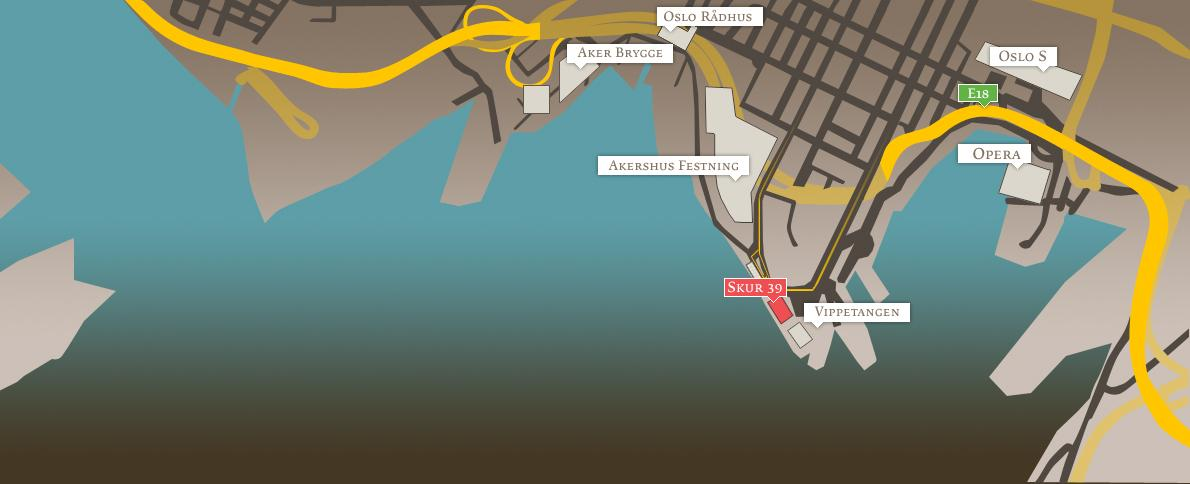
\includegraphics[height=11em]{bekk}
    \\\vspace{2em}\hfill\\
    \small
    
\includegraphics[height=1em]{bekk-logo}
    \\\vspace{.4em}\hfill\\
    \fontsize{8}{8}
    \selectfont
    \textbf{Aslak Johannessen}\\
    Senior Consultant\\
    982 19 249 \\
    aslakjo@bekk.no\\
    \vspace{.3em}\hfill\\
    \fontsize{1}{1}
    \selectfont
    BEKK CONSULTING AS\\
S   KUR 39, VIPPETANGEN. P.O. BOX 134 SENTRUM, 0102 OSLO, NORWAY. WWW.BEKK.NO\\
  \end{centering}
\end{frame}

\end{document}
